
%%% Preamble
\documentclass[paper=a4, fontsize=11pt]{scrartcl}
\usepackage[T1]{fontenc}
\usepackage{fourier}
\usepackage[utf8]{inputenc}
\usepackage[spanish]{babel}					% English language/hyphenation

\usepackage[protrusion=true,expansion=true]{microtype}	
\usepackage{amsmath,amsfonts,amsthm} % Math packages
\usepackage[pdftex]{graphicx}	
\usepackage{url}
\usepackage{import}

\usepackage[margin=2cm]{geometry}

% %%% Custom sectioning
\usepackage{sectsty}
\allsectionsfont{\normalfont \scshape}


%%% Custom headers/footers (fancyhdr package)
\usepackage{fancyhdr}
\pagestyle{fancyplain}
\fancyhead{}											% No page header
\fancyfoot[L]{}											% Empty 
\fancyfoot[C]{}											% Empty
\fancyfoot[R]{\thepage}									% Pagenumbering
\renewcommand{\headrulewidth}{0pt}			% Remove header underlines
\renewcommand{\footrulewidth}{0pt}				% Remove footer underlines
\setlength{\headheight}{13.6pt}


%%% Equation and float numbering
\numberwithin{equation}{section}		% Equationnumbering: section.eq#
\numberwithin{figure}{section}			% Figurenumbering: section.fig#
\numberwithin{table}{section}				% Tablenumbering: section.tab#


%%% Maketitle metadata
\newcommand{\horrule}[1]{\rule{\linewidth}{#1}} 	% Horizontal rule

%AGREGO PARA EJ 1
\usepackage{graphicx}
\usepackage{color} 
\usepackage[dvipsnames]{xcolor}
\colorlet{purple}{purple}

%/////////////////////////////////// AGREGO PARA EL EJ 2

    \usepackage{geometry} % Required to change the page size to A4
    \geometry{a4paper} % Set the page size to be A4 as opposed to the default US Letter

    \usepackage{mathtools, nccmath}
    
    \usepackage{tikz}
    \usetikzlibrary{matrix,calc}

    %isolated term
%#1 - Optional. Space between node and grouping line. Default=0
%#2 - node
%#3 - filling color
\newcommand{\implicantsol}[3][0]{
    \draw[rounded corners=3pt, fill=#3, opacity=0.3] ($(#2.north west)+(135:#1)$) rectangle ($(#2.south east)+(-45:#1)$);
    }


%internal group
%#1 - Optional. Space between node and grouping line. Default=0
%#2 - top left node
%#3 - bottom right node
%#4 - filling color
\newcommand{\implicant}[4][0]{
    \draw[rounded corners=3pt, fill=#4, opacity=0.3] ($(#2.north west)+(135:#1)$) rectangle ($(#3.south east)+(-45:#1)$);
    }

%group lateral borders
%#1 - Optional. Space between node and grouping line. Default=0
%#2 - top left node
%#3 - bottom right node
%#4 - filling color
\newcommand{\implicantcostats}[4][0]{
    \draw[rounded corners=3pt, fill=#4, opacity=0.3] ($(rf.east |- #2.north)+(90:#1)$)-| ($(#2.east)+(0:#1)$) |- ($(rf.east |- #3.south)+(-90:#1)$);
    \draw[rounded corners=3pt, fill=#4, opacity=0.3] ($(cf.west |- #2.north)+(90:#1)$) -| ($(#3.west)+(180:#1)$) |- ($(cf.west |- #3.south)+(-90:#1)$);
}

%group top-bottom borders
%#1 - Optional. Space between node and grouping line. Default=0
%#2 - top left node
%#3 - bottom right node
%#4 - filling color
\newcommand{\implicantdaltbaix}[4][0]{
    \draw[rounded corners=3pt, fill=#4, opacity=0.3] ($(cf.south -| #2.west)+(180:#1)$) |- ($(#2.south)+(-90:#1)$) -| ($(cf.south -| #3.east)+(0:#1)$);
    \draw[rounded corners=3pt, fill=#4, opacity=0.3] ($(rf.north -| #2.west)+(180:#1)$) |- ($(#3.north)+(90:#1)$) -| ($(rf.north -| #3.east)+(0:#1)$);
}

%group corners
%#1 - Optional. Space between node and grouping line. Default=0
%#2 - filling color
\newcommand{\implicantcantons}[2][0]{
    \draw[rounded corners=3pt, opacity=.3] ($(rf.east |- 0.south)+(-90:#1)$) -| ($(0.east |- cf.south)+(0:#1)$);
    \draw[rounded corners=3pt, opacity=.3] ($(rf.east |- 8.north)+(90:#1)$) -| ($(8.east |- rf.north)+(0:#1)$);
    \draw[rounded corners=3pt, opacity=.3] ($(cf.west |- 2.south)+(-90:#1)$) -| ($(2.west |- cf.south)+(180:#1)$);
    \draw[rounded corners=3pt, opacity=.3] ($(cf.west |- 10.north)+(90:#1)$) -| ($(10.west |- rf.north)+(180:#1)$);
    \fill[rounded corners=3pt, fill=#2, opacity=.3] ($(rf.east |- 0.south)+(-90:#1)$) -|  ($(0.east |- cf.south)+(0:#1)$) [sharp corners] ($(rf.east |- 0.south)+(-90:#1)$) |-  ($(0.east |- cf.south)+(0:#1)$) ;
    \fill[rounded corners=3pt, fill=#2, opacity=.3] ($(rf.east |- 8.north)+(90:#1)$) -| ($(8.east |- rf.north)+(0:#1)$) [sharp corners] ($(rf.east |- 8.north)+(90:#1)$) |- ($(8.east |- rf.north)+(0:#1)$) ;
    \fill[rounded corners=3pt, fill=#2, opacity=.3] ($(cf.west |- 2.south)+(-90:#1)$) -| ($(2.west |- cf.south)+(180:#1)$) [sharp corners]($(cf.west |- 2.south)+(-90:#1)$) |- ($(2.west |- cf.south)+(180:#1)$) ;
    \fill[rounded corners=3pt, fill=#2, opacity=.3] ($(cf.west |- 10.north)+(90:#1)$) -| ($(10.west |- rf.north)+(180:#1)$) [sharp corners] ($(cf.west |- 10.north)+(90:#1)$) |- ($(10.west |- rf.north)+(180:#1)$) ;
}

%Empty Karnaugh map 4x4
\newenvironment{Karnaugh}%
{
\begin{tikzpicture}[baseline=(current bounding box.north),scale=0.8]
\draw (0,0) grid (4,4);
\draw (0,4) -- node [pos=0.7,above right,anchor=south west] {AB} node [pos=0.75,below left,anchor=north east] {CD} ++(135:1);
%
\matrix (mapa) [matrix of nodes,
        column sep={0.8cm,between origins},
        row sep={0.8cm,between origins},
        every node/.style={minimum size=0.3mm},
        anchor=8.center,
        ampersand replacement=\&] at (0.5,0.5)
{
                       \& |(c00)| 00         \& |(c01)| 01         \& |(c11)| 11         \& |(c10)| 10         \& |(cf)| \phantom{00} \\
|(r00)| 00             \& |(0)|  \phantom{0} \& |(1)|  \phantom{0} \& |(3)|  \phantom{0} \& |(2)|  \phantom{0} \&                     \\
|(r01)| 01             \& |(4)|  \phantom{0} \& |(5)|  \phantom{0} \& |(7)|  \phantom{0} \& |(6)|  \phantom{0} \&                     \\
|(r11)| 11             \& |(12)| \phantom{0} \& |(13)| \phantom{0} \& |(15)| \phantom{0} \& |(14)| \phantom{0} \&                     \\
|(r10)| 10             \& |(8)|  \phantom{0} \& |(9)|  \phantom{0} \& |(11)| \phantom{0} \& |(10)| \phantom{0} \&                     \\
|(rf) | \phantom{00}   \&                    \&                    \&                    \&                    \&                     \\
};
}%
{
\end{tikzpicture}
}

%Empty Karnaugh map 2x4
\newenvironment{Karnaughvuit}%
{
\begin{tikzpicture}[baseline=(current bounding box.north),scale=0.8]
\draw (0,0) grid (4,2);
\draw (0,2) -- node [pos=0.7,above right,anchor=south west] {bc} node [pos=0.7,below left,anchor=north east] {a} ++(135:1);
%
\matrix (mapa) [matrix of nodes,
        column sep={0.8cm,between origins},
        row sep={0.8cm,between origins},
        every node/.style={minimum size=0.3mm},
        anchor=4.center,
        ampersand replacement=\&] at (0.5,0.5)
{
                      \& |(c00)| 00         \& |(c01)| 01         \& |(c11)| 11         \& |(c10)| 10         \& |(cf)| \phantom{00} \\
|(r00)| 0             \& |(0)|  \phantom{0} \& |(1)|  \phantom{0} \& |(3)|  \phantom{0} \& |(2)|  \phantom{0} \&                     \\
|(r01)| 1             \& |(4)|  \phantom{0} \& |(5)|  \phantom{0} \& |(7)|  \phantom{0} \& |(6)|  \phantom{0} \&                     \\
|(rf) | \phantom{00}  \&                    \&                    \&                    \&                    \&                     \\
};
}%
{
\end{tikzpicture}
}

%Empty Karnaugh map 2x2
\newenvironment{Karnaughquatre}%
{
\begin{tikzpicture}[baseline=(current bounding box.north),scale=0.8]
\draw (0,0) grid (2,2);
\draw (0,2) -- node [pos=0.7,above right,anchor=south west] {b} node [pos=0.7,below left,anchor=north east] {a} ++(135:1);
%
\matrix (mapa) [matrix of nodes,
        column sep={0.8cm,between origins},
        row sep={0.8cm,between origins},
        every node/.style={minimum size=0.3mm},
        anchor=2.center,
        ampersand replacement=\&] at (0.5,0.5)
{
          \& |(c00)| 0          \& |(c01)| 1  \\
|(r00)| 0 \& |(0)|  \phantom{0} \& |(1)|  \phantom{0} \\
|(r01)| 1 \& |(2)|  \phantom{0} \& |(3)|  \phantom{0} \\
};
}%
{
\end{tikzpicture}
}

%Defines 8 or 16 values (0,1,X)
\newcommand{\contingut}[1]{%
\foreach \x [count=\xi from 0]  in {#1}
     \path (\xi) node {\x};
}

%Places 1 in listed positions
\newcommand{\minterms}[1]{%
    \foreach \x in {#1}
        \path (\x) node {1};
}

%Places 0 in listed positions
\newcommand{\maxterms}[1]{%
    \foreach \x in {#1}
        \path (\x) node {0};
}

%Places X in listed positions
\newcommand{\indeterminats}[1]{%
    \foreach \x in {#1}
        \path (\x) node {X};
}

    \linespread{1.2} % Line spacing
    
    \setlength\parindent{0pt} % Uncomment to remove all indentation from paragraphs
    
   % \graphicspath{{/home/bzerol/VisualCode/ElectroIII/tp1-team-2/E2TP1}} % Specifies the directory where pictures are stored

%//////////////////////////////////// agrego para EJ 4
%\documentclass[english]{article}
%\usepackage[T1]{fontenc}
%\usepackage[latin9]{inputenc}
%\usepackage{geometry}
%\geometry{verbose,tmargin=2cm,bmargin=2cm,lmargin=2cm,rmargin=2cm,headheight=2cm,headsep=2cm}
%\usepackage{float}
%\usepackage{graphicx}

\makeatletter

%%%%%%%%%%%%%%%%%%%%%%%%%%%%%% LyX specific LaTeX commands.
%% Because html converters don't know tabularnewline
\providecommand{\tabularnewline}{\\}

%%%%%%%%%%%%%%%%%%%%%%%%%%%%%% User specified LaTeX commands.
\usepackage{babel}


\makeatother

\usepackage{babel}

\usepackage{tikz}
\usepackage{circuitikz}
%\usemodule[circuitikz]
%\usepackage{circuitikzgit}



%///////////////////////////// PARA EL EJ6
%\documentclass[english]{article}
%\usepackage[T1]{fontenc}
%\usepackage[latin9]{inputenc}
%\usepackage{geometry}
%\geometry{verbose,tmargin=3cm,bmargin=3cm,lmargin=3cm,rmargin=3cm,headheight=3cm,headsep=3cm}
%\usepackage{float}

%\makeatletter

%%%%%%%%%%%%%%%%%%%%%%%%%%%%%% LyX specific LaTeX commands.
%% Because html converters don't know tabularnewline
\providecommand{\tabularnewline}{\\}








%%% Begin document
\begin{document}

\title{
	%\vspace{-1in}
	\usefont{OT1}{bch}{b}{n}
	\normalfont \normalsize \textsc{Instituto Tecnológico de Buenos Aires} \\ [25pt]
	\horrule{2pt} \\[0.4cm]
	\huge Trabajo de Laboratorio \\
	\horrule{2pt} \\[0cm]
\author{Grupo 2:\\Díaz Ian Cruz\\Mestanza Nicol\'as\\ Müller Malena\\Rodr\'iguez Turco Mart\'in\\ Scala Tob\'ias\\ \\ }
\text{F\'isica Electrónica - 2019}
}
\date{\today} %ver si dejar la de today o poner fecha fija que sea August 2018
\pagenumbering{arabic}

\maketitle
\newpage

% The \input command appends the content of the file directly into the document.
\section*{\color{olive}Ejercicio 1: Medici\'on de curvas caracter\'isticas de diodos}

\begin{figure}[h!]
 \begin{center}
    \begin{circuitikz}
    \draw (0,3)
	%(0,0) node[ground] {}
      to[V,v=$V_{cc}$] (0,0) % The voltage source
	(0,3) to[Do] (2,3)
%  (0,3) to[short] (1,3) node[fulldiodeshape]{} 
%	(1,3) to[short] (2,3)
      to[R=$R_1$] (2,0) % The resistor
	to[short] (2,0)
	to[short] (1,0) node[ground]{}
	(1,0) to[short] (0,0);

    \draw (6,3)
	%(0,0) node[ground] {}
      to[V,v=$V_{cc}$] (6,0) % The voltage source
	(6,3) to[zDo] (8,3)
%  (0,3) to[short] (1,3) node[fulldiodeshape]{} 
%	(1,3) to[short] (2,3)
      to[R=$R_1$] (8,0) % The resistor
	to[short] (8,0)
	to[short] (7,0) node[ground]{}
	(7,0) to[short] (6,0);

    \draw (12,3)
	%(0,0) node[ground] {}
      to[V,v=$V_{cc}$] (12,0) % The voltage source
	(12,3) to[leDo] (14,3)
%  (0,3) to[short] (1,3) node[fulldiodeshape]{} 
%	(1,3) to[short] (2,3)
      to[R=$R_1$] (14,0) % The resistor
	to[short] (14,0)
	to[short] (13,0) node[ground]{}
	(14,0) to[short] (12,0);
    \end{circuitikz}

    \caption{\color{cyan}Circuitos empleados para medir la curva caracter\'istica de un diodo rectificador, de un diodo zener y de un LED; respectivamente.}
\end{center}
\end{figure}

%%% diodo rectificador
\subsection*{\color{orange}Diodo rectificador}

A continuaci\'on se presentan los gr\'aficos de la corriente vs. tensi\'on para el caso del diodo rectificador 1N4148. 

\begin{figure}[!ht]
\centering
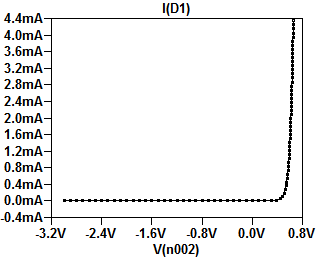
\includegraphics[scale=0.62]{../EJ1/DiodoRectificador/corrienteDiodo1}
\caption{Simulaci\'on corriente vs. tensi\'on del diodo rectificador.}
\label{med1a}
\end{figure}

\begin{figure}[!ht]
\centering
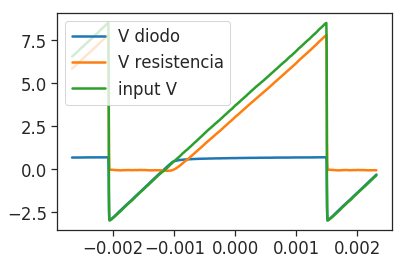
\includegraphics[scale=0.5]{../EJ1/DiodoRectificador/datosOsciloscopio}
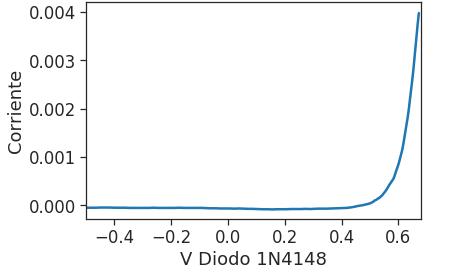
\includegraphics[scale=0.5]{../EJ1/DiodoRectificador/diodoRectMedido}
\caption{Medici\'on de la corriente vs. tensi\'on del diodo rectificador: Datos obtenidos y datos procesados; respectivamente.}
\label{med1b}
\end{figure}

\begin{figure}[!ht]
\centering
\includegraphics[scale=0.52]{../EJ1/DiodoRectificador/corrienteDiodoDatasheet}
\caption{Corriente vs. tensi\'on del diodo rectificador obtenida de la hoja de datos.}
\label{med1c}
\end{figure}

%%% diodo zener
\subsection*{\color{orange}Diodo zener}

\begin{figure}[H]
\centering
\includegraphics[scale=0.62]{../EJ1/DiodoZener/simulacionZener}
\caption{Simulaci\'on corriente vs. tensi\'on del diodo zener.}
\label{med2a}
\end{figure}

\begin{figure}[H]
\centering
\includegraphics[scale=0.5]{../EJ1/DiodoZener/datosOsciloscopioZener}
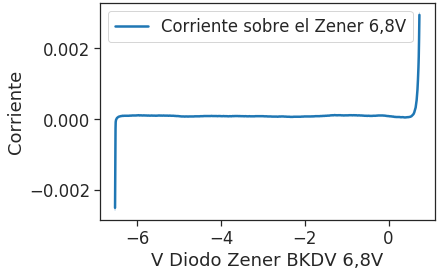
\includegraphics[scale=0.5]{../EJ1/DiodoZener/zenerMedido}
\caption{Medici\'on de la corriente vs. tensi\'on del diodo zener: Datos obtenidos y datos procesados; respectivamente.}
\label{med2b}
\end{figure}

%\begin{figure}[!ht]
%\centering
%\includegraphics[scale=0.52]{../EJ1/DiodoZener/corrienteDiodoDatasheet}
%\caption{Corriente vs. tensi\'on del diodo zener obtenida de la hoja de datos.}
%\label{med2c}
%\end{figure}

%%% led
\subsection*{\color{orange}LED}

%\begin{figure}[H]
%\centering
%\includegraphics[scale=0.62]{../EJ1/LED/simulacionZener}
%\caption{Simulaci\'on corriente vs. tensi\'on del LED.}
%\label{med3a}
%\end{figure}

%\begin{figure}[H]
%\centering
%\includegraphics[scale=0.5]{../EJ1/LED/datosOsciloscopioZener}
%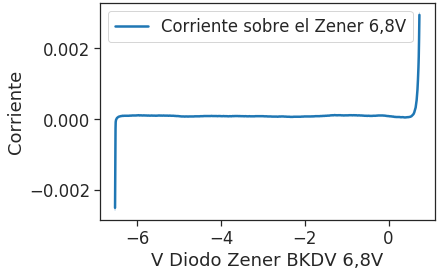
\includegraphics[scale=0.5]{../EJ1/DiodoZener/zenerMedido}
%\caption{Medici\'on de la corriente vs. tensi\'on del LEDr: Datos obtenidos y datos procesados; respectivamente.}
%\label{med3b}
%\end{figure}

%\begin{figure}[!ht]
%\centering
%\includegraphics[scale=0.52]{../EJ1/LED/corrienteDiodoDatasheet}
%\caption{Corriente vs. tensi\'on del LED obtenida de la hoja de datos.}
%\label{med3c}
%\end{figure}

\section*{\color{olive}Ejercicio 2: C\'alculo y simulaci\'on de una funci\'on transferencia de tensi\'on}

\begin{figure}[H] %!ht
 \begin{center}
    \begin{circuitikz}[american]
    \draw (0,3) to[sV,v=$V_{in}$] (0,0) % The voltage source
(0,3)  to[short] (1,3) to[R, l2_=$R_G$ and $50\Omega$] 
(2,3)  to[short] (3,3) to[C=$C_{in}$] (4,3) to[short] (5.5,3) 
%to[R=$R_G$]  (2,3)  to[short] (3,3) to[C=$c_{in}$] (4,3) to[short] (5.5,3) 
(6,3) node[npn]{}
(0,0) to[short] (6,0) to[R=$R_E$] (6,2.5)
(4.5,0) to[R=$R_2$] (4.5,3) to[R=$R_1$] (4.5,6) to[short] (6,6) to[R=$R_C$] (6,3.5)
 to[C=$C_{out}$] (9,3.5) node[anchor=west] {OUT} (9,3.5)
 to[R=$R_L$] (9,0) to[short] (6,0)
(7.5,0) to[pC=$C_E$] (7.5,2.5) to[short] (6,2.5)
(4.5,6)  to[V, v=$V_{cc}$] (0,6) node[ground]{}
(2.5,3) node[anchor=south] {IN} 
(4.5,0) node[ground]{};
    \end{circuitikz}
    \caption{Circuito con un transistor NPN BC547B, para el cual se obtiene la funci\'on transferencia.}
	\label{circ2}
\end{center}
\end{figure}


Siendo
%\begin{itemize}
%\item $ R_1 = 100k\Omega$
%\item $ R_2 = 27k\Omega$
%\item $ R_C = 11.2k\Omega$
%\item $ R_E = 3k\Omega$
%\item $ R_L = 10k\Omega$
%\item $ C_{in} = 20nF$
%\item $ C_{out} = 10nF$
%\item $ C_E = 2\mu F$
%\end{itemize}

\begin{multicols}{4}
\begin{itemize}
\item $ R_1 = 100k\Omega$
\item $ R_2 = 27k\Omega$
\end{itemize}
\columnbreak
\begin{itemize}
\item $ R_C = 11.2k\Omega$
\item $ R_L = 10k\Omega$
\end{itemize}
\columnbreak
\begin{itemize}
\item $ R_E = 3k\Omega$
\item $ C_E = 2\mu F$
\end{itemize}
\columnbreak
\begin{itemize}
\item $ C_{in} = 20nF$
\item $ C_{out} = 10nF$
\end{itemize}
\end{multicols}


\subsection*{\color{orange} C\'alculo de la funci\'on transferencia de tensi\'on}

Para calcular la funci\'on transferencia de tensi\'on del circuito \ref{circ2}, se utiliza el modelo h\'ibrido $\pi$ como circuito equivalente del transistor NPN en peque\~na se\~nal, pasivando la fuente de tensi\'on cont\'inua. Adem\'as, a muy bajas frecuencias se considera que los capacitores se comportan como cortocircuitos. El siguiente circuito es el equivalente correspondiente al circuito \ref{circ2}:

\begin{figure}[H]%!ht
 \begin{center}
    \begin{circuitikz}[american]
    \draw (0,1.5) to[sV,v=$V_{in}$] (0,0) % The voltage source
(0,1.5) to[R=$R_G$] (0,3)
(2,0) to[R=$R_1$] (2,3)
(4,0) to[R=$R_2$] (4,3)
(6,0) to[R=$R_{\pi}$] (6,3)
(8,3) to[cI=$I_1$] (8,0)
(10,0) to[R=$R_0$] (10,3)
(12,0) to[R=$R_C$] (12,3)
(14,0) to[R=$R_L$] (14,3)
	
(0,0) to[short] (14,0)
(0,3) to[short] (6,3)
(8,3) to[short] (14,3)
(7,0) node[ground]{}
(1,3) node[anchor=south] {IN} 
(14,3) node[anchor=west] {OUT};
    \end{circuitikz}
    \caption{Circuito equivalente empleado para el c\'alculo de la funci\'on transferencia de tensi\'on.}
	\label{circ22}
\end{center}
\end{figure}

A partir del circuito \ref{circ22}, surge que:
\begin{equation}\frac{V_{OUT}}{V_{IN}} = \frac{\left( R_0 // R_C // R_L\right) \beta}{ R_{\pi}} = \frac{R_L \cdot (R_0 + R_C) \cdot \beta}{R_{\pi} \cdot (R_0 R_C R_L + R_0 + R_C)} \label{ec1} \end{equation}

A partir de la simulaci\'on, medimos la impedancia de salida del circuito de la figura \ref{circ2} y obtuvimos el valor de $R_0$ del transistor NPN BC547B:\\
$R_0 = 103 \cdot k\Omega$\\
A su vez, usando el resto de los valores con los que est\'a modelada la simulaci\'on:\\
$R_{\pi} = 12,3 k\Omega$\\
$\beta = 294$

Con los valores anteriores, reemplazando en la ecuaci\'on \ref{ec1} se obtiene que:
$$ \frac{V_{OUT}}{V_{IN}} = 2.366\mu $$

Entonces:

\begin{equation} |\frac{V_{OUT}}{V_{IN}} |_{db} = -112 dB \label{ec2} \end{equation}

\subsection*{\color{orange} Simulaci\'on de la funci\'on transferencia de tensi\'on}


\begin{figure}[H] %!ht
\centering
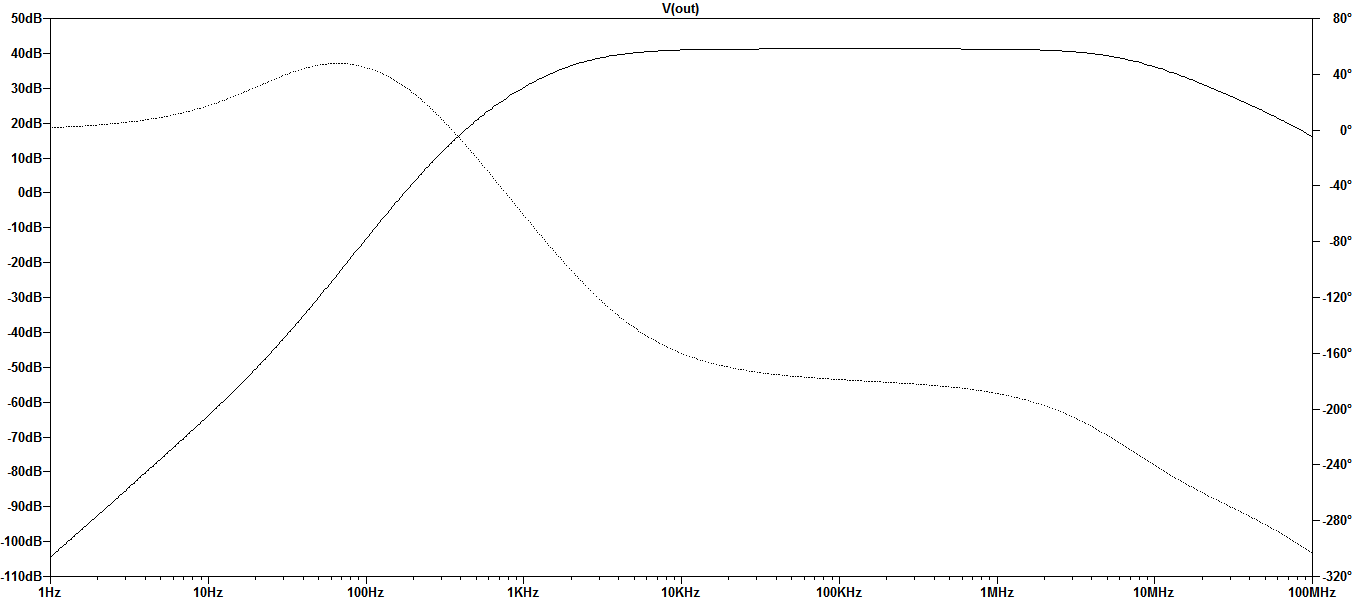
\includegraphics[scale=0.45]{../EJ2/rtaenfrec}
\caption{Simulaci\'on del circuito \ref{circ2}}
\label{simEj2}
\end{figure}

En la simulaci\'on de la figura \ref{simEj2}, la l\'inea oscura corresponde al m\'odulo de la funci\'on transferencia, mientras que la clara corresponde a su fase. A partir de la l\'inea oscura, se puede ver que a bajas frecuencias, como se modelo el circuito equivalente de pequeña señal, el valor obtenido en la ecuaci\'on \ref{ec2} coincide con la ganancia vista en el diagrama de Bode de la figura \ref{simEj2}




















\section*{\color{olive}Ejercicio 3: Simulaci\'on de la respuesta en frecuencia de un circuito en condiciones iniciales}

%\input{../E4TP1/E4TP1.tex}
%\input{../E5TP1/E5TP1.tex}
%\input{../E6TP1/E6TP1.tex}
%\input{appendix.tex}
%

%%% End document
\end{document}
